\chapter{Theory}

Two of the studies presented within this thesis are for prospective measurements looking at the $H\rightarrow WW$ branching ratio and the forward-backward asymmetry in \ttbar~ production at CLIC during the 1.4~TeV stage. As such it is important to first examine the significance of these measurements in the context of the physics programme of CLIC and the wider state of partile physics.


\section{Higgs Physics}

\begin{figure}
  \centering
  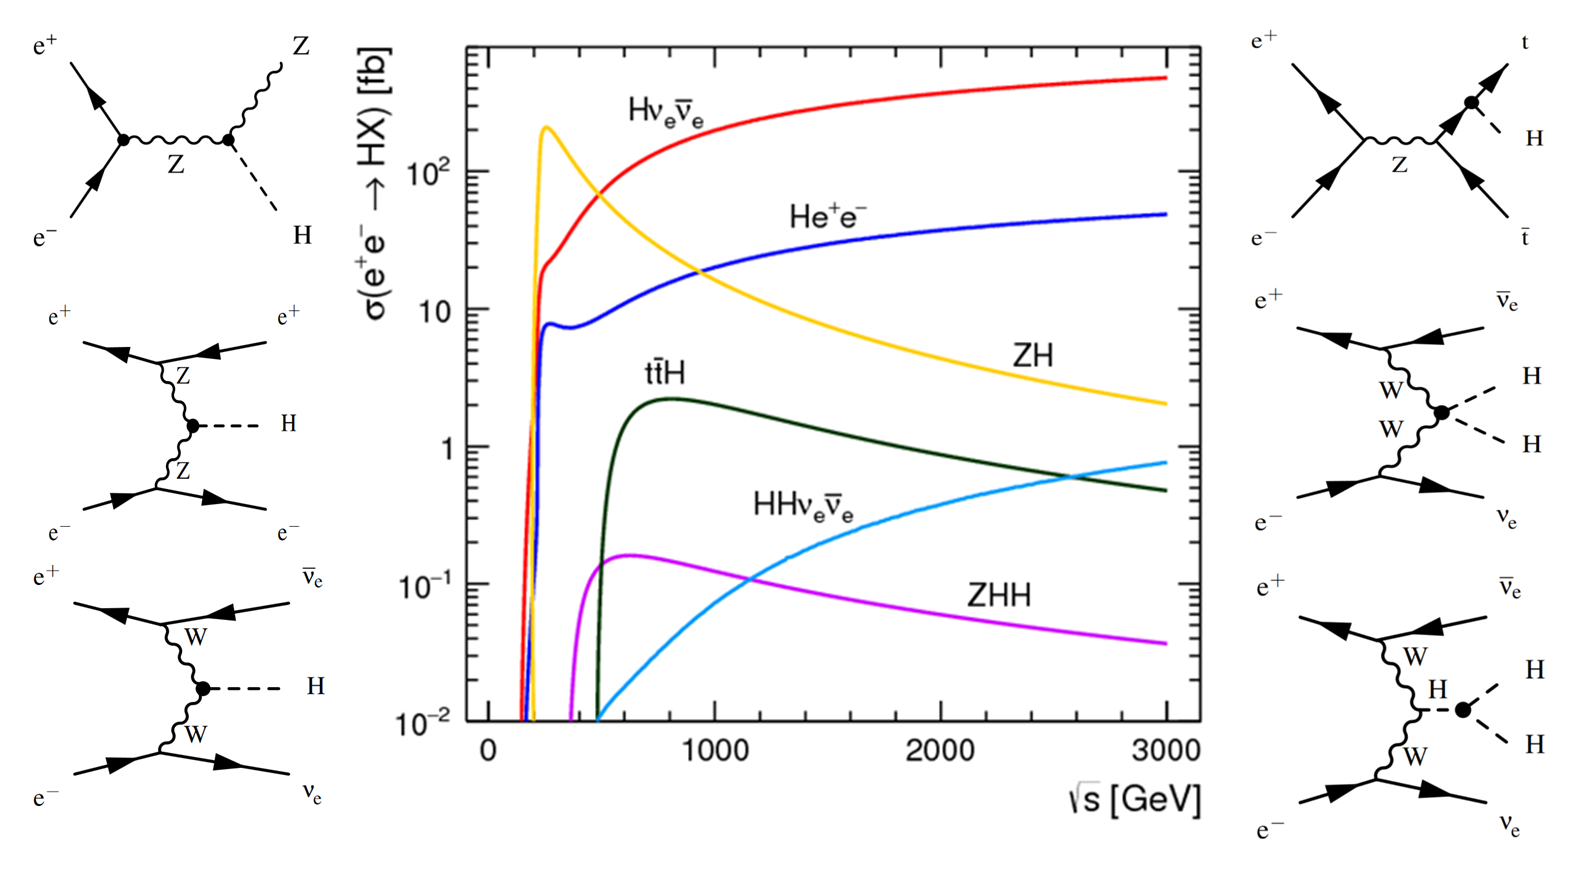
\includegraphics[width=0.95\textwidth,keepaspectratio]{Theory/fig/HiggsProcessesExtra.png}
  \caption[Cross Sections For Higgs Production Mechanisms]{Cross Sections For Higgs Production Mechanisms}
  \label{fig:higgsXSecs}
\end{figure}

The CLIC physics programme has a large focus on characterising the Higgs boson due to the large uncertainties on many of it's associated properties relative to other sectors of the standard model. In particluar it will aim to measure the mass, width, spin and couplings of the Higgs in a model independent manner. Electron positron collisions provide access to numerous Higgs production mechanisms which can be seen in \ref{fig:higgsXSecs}. Due to the strong energy dependence on many of the cross sections on energy, different processes will be of interest at each of the three energy stages operated at CLIC. At 380GeV the focus will predominantly be on measuring the Higgsstrahlung ($ZH$) process, while at higher energies vector boson fusion ($H\nu\nu,Hee$) dominates and new processes such as di-Higgs production become accessible. A summary of all the results from current Higgs studies performed by CLIC is available in \cite{Abramowicz:2016zbo}.

\subsection{Higgsstrahlung}

\begin{figure}
  \centering
  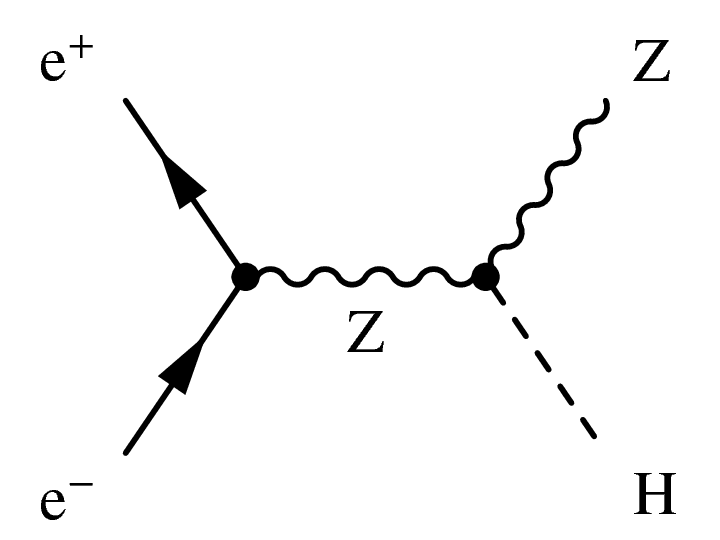
\includegraphics[width=0.45\textwidth,keepaspectratio]{Theory/fig/HiggsStrahlung.png}
  \caption[The Higgstrahlung Process]{The Higgstrahlung Process}
  \label{fig:higgsstrahlung}
\end{figure}


One of the key aims of the experiment will be to examine the Higgsstrahlung process shown in \ref{fig:higgsstrahlung}. In this process, if the four momentum of the Z boson can be measured to high precision, then because the initial conditions of the collision are well known, one can determine the mass of the particle it is recoling against ($m_{rec}^{2} = s + m_{z}^{2} - 2E_{z}^{2}$) and infer the presence of the Higgs. This allows properties such as the Higgs mass, cross-section and coupling to the Z to be measured without actually ever measuring the decay products of the Higgs boson which in turn allows the measurements to be model independent as few assumptions must be made about the interactions of the Higgs. This method is not possible at hadron colliders such as the LHC where, even though the Higgsstrahlung process still occurs, as the four momentum of the colliding particles can never be known to as high a level of precision due to their composite nature. Using the clean signal from cases where the Z decays to a pair of muons or electrons it is possible to measure the recoil mass to high precision and thus determine the mass of the Higgs to $\Delta m_{H} = 110~MeV$ (see figure \ref{fig:higgsmass} using data from the low energy stage only. This value can be further improved to $\Delta m_{H} = 44~MeV$ when including direction measurement results from the $ee\rightarrow H\nu\bar{\nu}, H\rightarrow b\bar{b}$ channel at 3~TeV. Despite giving a poorer resolution on the Z four momentum, the $Z\rightarrow qq$ higgsstrahlung channel is also considered due to it's larger cross section. Using this channel a limit of $BR(H\rightarrow invis.) <0.97\%$ at 90\% C.L. can be set. 

\begin{figure}
  \centering
  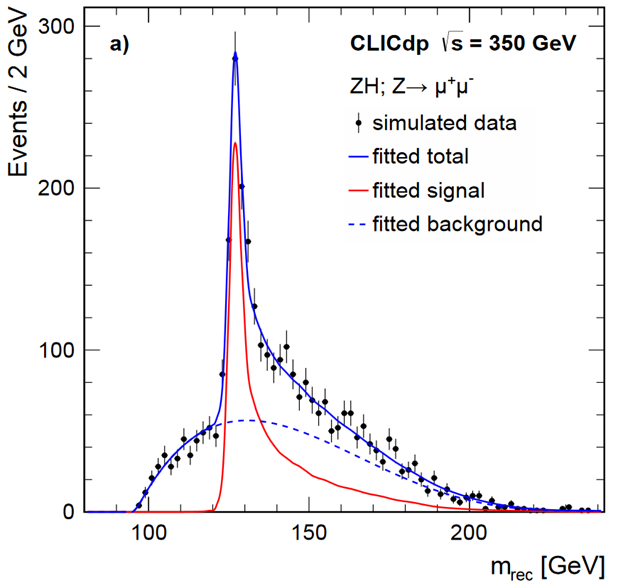
\includegraphics[width=0.45\textwidth,keepaspectratio]{Theory/fig/HiggsRecoilMass.png}
  \caption[Reconstructed recoil mass from Higgsstralung process]{Reconstructed recoil mass from Higgsstralung process}
  \label{fig:higgsstrahlung}
\end{figure}

 
\subsection{Model Independent Extraction of Higgs Couplings}


While the Higgsstrahlung alone allows the mass and branching ratios of the Higgs to be determined, by measuring the rates of several different Higgs processes and combining them in the right ratio, it is further possible to extract the absolute width of the Higgs. One such ``recipe'' proposed for doing this is shown in \ref{modelindependentformula} \cite{Durig:2014lfa}:


\begin{equation}
  \label{modelindependentformula}
  \Gamma_H = \frac{Y_1^2Y_3^2}{Y_4^2Y_2}
\end{equation}

where

\begin{equation}
X_1=\sigma_{ZH} \propto g_{HZZ}^2
\end{equation}

\begin{equation}
  \label{X2}
  X_2=\sigma_{H\nu\bar{\nu}} \times BR(H\rightarrow WW^*) \propto \frac{g_{HWW}^4}{\Gamma_H}
\end{equation}

\begin{equation}
X_3=\sigma_{H\nu\bar{\nu}} \times BR(H\rightarrow b\bar{b}) \propto \frac{g_{HWW}^{2}g_{Hbb}^2}{\Gamma_H}
\end{equation}

\begin{equation}
X_4=\sigma_{ZH} \times BR(H\rightarrow b\bar{b}) \propto \frac{g_{HZZ}^{2}g_{Hbb}^2}{\Gamma_H}
\end{equation}


Currently at the LHC the standard process for extracting couplings from the equivalent measurements of $X_{2,3\&4}$ is to multiply through by the standard model value of the Higgs width. This type of measurement is referred to as `model-dependent` as the values determined for the Higgs couplings carry the implicit assumption that the standard model is correct in it's prediction of the Higgs width. At CLIC, because the width can be measured experimentally there is no need to make this assumption and so the couplings are measured in a ``model-independent'' way. The unique ability of linear colliders to perform model-independent measurements is one of the largest driving factors for constructing and using them as a so called ``Higgs-Factory''. One limiting factor for the model-independent measurements of the couplings is that they are always ultimately dependent on the precision to which the ZH cross section can be measured (predicted to be $\Delta h_{HZZ} = 0.8\%$) as this quantity is always needed in the ratio used to extract $\Gamma_H$. With the exception of $X_1$, the choice of variables used is not unique (e.g. one could replace the production mechanism in $X_1$ and $X_2$ with ZZ-fusion rather than WW-fusion,) however the combination shown here is expected to give the highest precision on $\Gamma_H$ due to the large cross-section associated with WW-fusion and the high branching ratio of $H\rightarrow b\bar{b}$ ($\sim$ 65\%). In chapter \ref{Higgs Analysis} we will present our research on the precision to which $X_2$ from eq \ref{X2} can be measured during the 1.4~TeV run at CLIC.

In practice it is expected that an 11 parameter global fit to multiple variations of these measurements will be performed at each stage of operation to extract the Higgs width and it's couplings to both fermions and bosons. The relevant inputs for these fits are shown in tables (INSERT table 28 and 29 from higgs paper) while the results of the fits are shown in (table 26 and fig 28 from higgs paper.)



For context it is also important to compare these results to what can be expected from current leading experiments such as ATLAS and CMS at the LHC and what is necessary to test relevant theories.

Explain that we need to compare model-dependent results- show change in results from CLIC alone (fig 26 and 27 from higgs paper) and the show the comparison to LHC predictions

Show snow mass plot from phil burrows talk to emphasise that theory predictions are of the saem order that CLIC can manage but not LHC. 

\section{Top Quark Physics}

Define what the forward backward asymmetry is, brief history of measurents elsewhere

How it can be used to measure EW couplings

New physics that can effect these couplings e.g. Z'



AFB
EW Couplings
%Mass
%Width


